\subsection{Pruebas Individuales de Componentes con Arduino }
\par \noindent
Todas las pruebas serán utilizando un arduino nano; ya que permite una integración sencilla con un breadboard y sera el que utilizaremos en nuestro prototipo final. Empezaremos con el sensor de temperatura DS18B20.

\subsubsection{Arduino y DS18B20}
\par 
Si leemos detenidamente el datasheet del DS18B20 podemos encontrar que es mas complejo que un simple termopar para medir la temperatura. Cuenta en su forma de sonda con distintos circuitos integrados que permiten la facil integración con arduino. El DS18B20 utiliza tres alambres. Uno para la alimentación de 5V, otro para tierra y uno de información o data. Este ultimo es conectado a traves de una resistencia de 4.7K ohmnios en parallelo con una alimentación de 5V y cualquier pin digital de arduino. 

\begin{figure}[H]
	\centering
	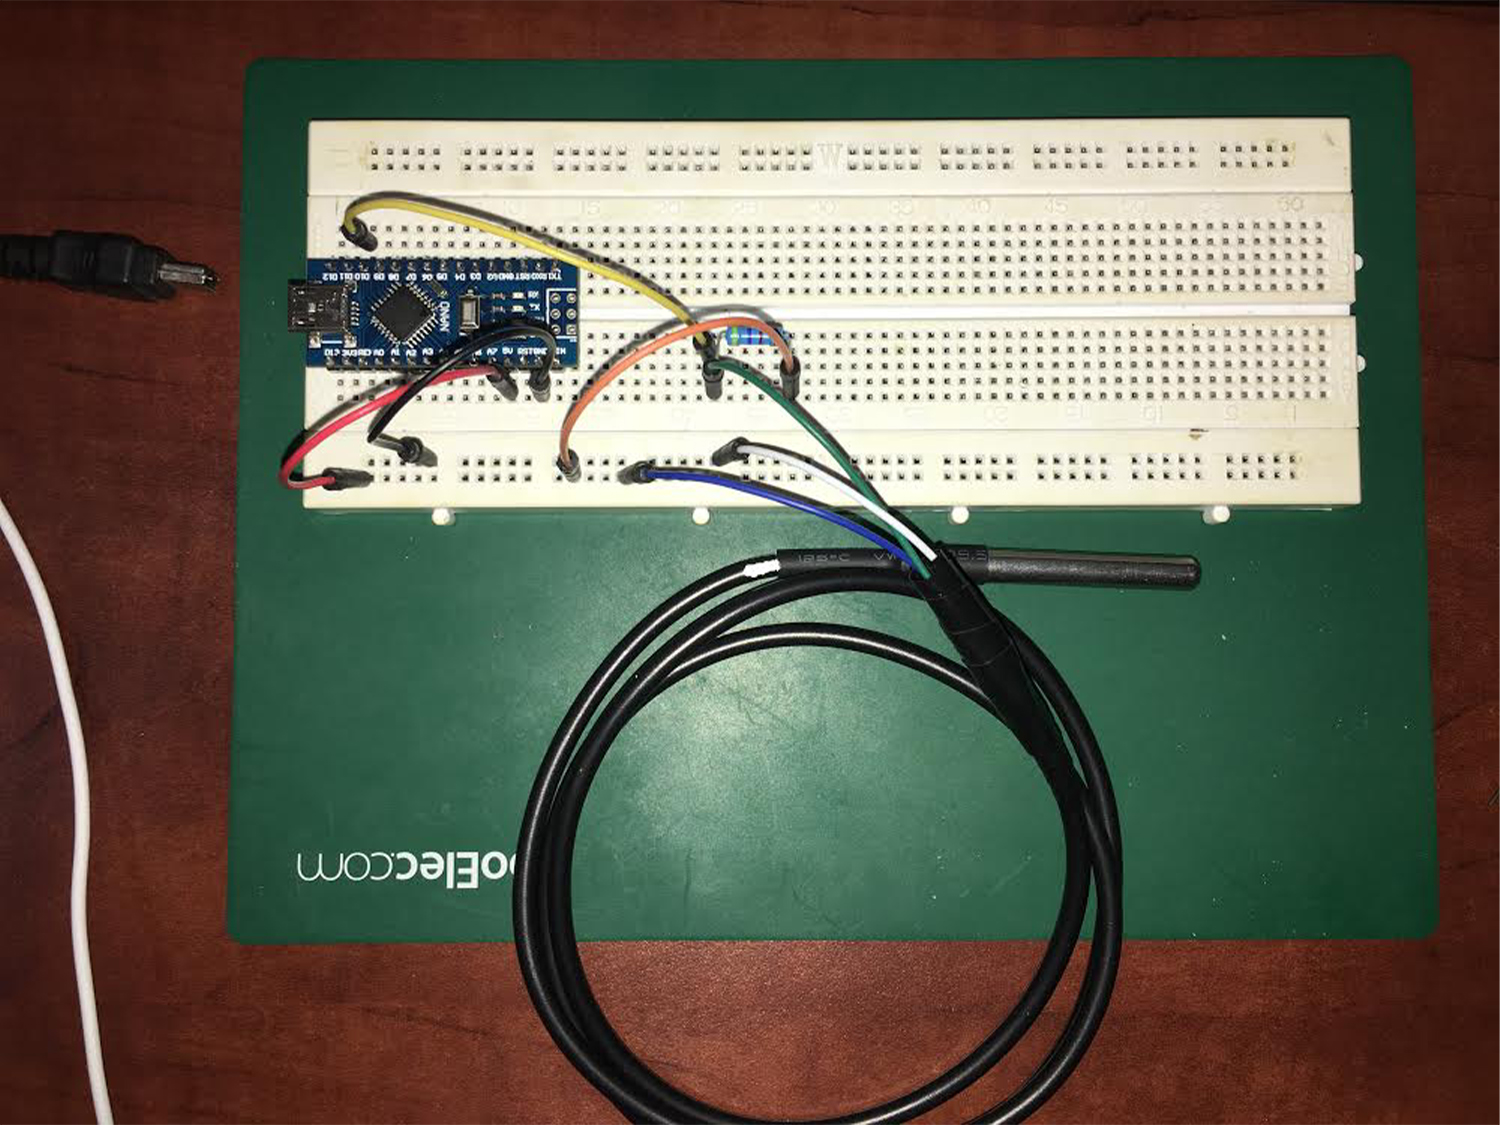
\includegraphics[width=0.65\linewidth]{pruebas1.jpg}
	\caption{Conexión Sencilla entre Arduino Nano y Sensor de Temperatura DS18B20}
\end{figure}

\par \noindent
En la imagen anterior hemos seleccionado el pin digital 10 para enviar la información y vemos como el sensor es conectado a la salida de 5V del Arduino y su respectivo GND, adicional vemos una resistencia de 4.7K entre el cable de DATA del sensor y una conexión al pin 10. 

\par \noindent
Ahora utilizando el software platformio, el entorno de desarrollo que utilizaremos para programar la placa arduino, escribiremos un codigo de prueba. Para ellos necesitaremos de dos librerias: OneWire \cite{onewire-github} y DallasTemperature \cite{dallas-github}. El código de prueba seria el siguiente: \\

\begin{lstlisting}[language=C++, caption={Codigo Ejemplo para DS18B20}, captionpos=b]
#include <Arduino.h>
#include <OneWire.h>
#include <DallasTemperature.h>

#define ONE_WIRE_BUS 10

OneWire oneWire(ONE_WIRE_BUS);
DallasTemperature sensors(&oneWire);

void setup(){
	Serial.begin(9600);
 	sensors.begin();
}


void loop(){
	Serial.print("Requesting temperatures...");
	sensors.requestTemperatures(); 
	Serial.println("DONE");
	Serial.print("Temperature:");
	Serial.println(sensors.getTempCByIndex(0));
	delay(1000);
}
\end{lstlisting}

\par \noindent
El codigo anterior puede ser encontrado como uno de los ejemplos que trae la libreria DallasTemperature\cite{dallas-github} bajo el nombre "Simple.pde" y puede inspeccionado por cualquier editor de texto.

\clearpage

\par \noindent
Una vez hayamos subido el codigo a nuestro Arduino, debemos validar que el sensor funcione correctamente pero ¿como? Conectado el Arduino a nuestra computadora utilizaremos el puerto serial de nuestro entorno de desarrollo. Si estamos utilizando el IDE de arduino, basta con hacer click en la barra superior la opcion "herramientas" y seleccionar "Monitor Serial". Como nosotros estamos utilizando Platformio como IDE, basta con seleccionar en la barra de herramientas "Platformio", la opción "Serial Monitor". Esencialmente lo que hace esa opción es escribir en nuestra terminal el comando 
"pio device monitor --port COM5" y con eso podemos comunicarnos con nuestro Arduino a través de un puerto Serial.